%%%%  TEIL II: PHYSIK LESEN UND SPRECHEN  %%%%
\newpage
\part{Physik lesen und sprechen}

In diesem Teil steht, wie man Einheiten, Größenangaben und Formeln auf Englisch (und zum Vergleich
auf Deutsch) vorliest und wie man Experimente und Diagramme beschreibt. Links steht der Ausdruck,
rechts die englische Lesart und darunter grau die deutsche.

%--------------------------------------------------------------------------------------------------
\section{Die Basiseinheiten des SI}

Das Internationale Einheitensystem (\textit{International System of Units}, SI) hat sieben
Basiseinheiten. Alle anderen Einheiten werden daraus abgeleitet.

\begin{lesen}
\lies{$\mathrm{m}$}{metre \ipa{"mi:t@} (AE: meter) -- the unit of length}{Meter -- die Einheit der Länge}
\lies{$\mathrm{kg}$}{kilogram \ipa{"kIl@gr\ae m} -- the unit of mass}{Kilogramm -- die Einheit der Masse}
\lies{$\mathrm{s}$}{second \ipa{"sek@nd} -- the unit of time}{Sekunde -- die Einheit der Zeit}
\lies{$\mathrm{A}$}{ampere \ipa{"\ae mpe@} (short: amp) -- the unit of electric current}{Ampere -- die Einheit der elektrischen Stromstärke}
\lies{$\mathrm{K}$}{kelvin \ipa{"kelvIn} -- the unit of thermodynamic temperature}{Kelvin -- die Einheit der absoluten Temperatur}
\lies{$\mathrm{mol}$}{mole \ipa{m@Ul} -- the unit of amount of substance}{Mol -- die Einheit der Stoffmenge}
\lies{$\mathrm{cd}$}{candela \ipa{k\ae n"del@} -- the unit of luminous intensity}{Candela -- die Einheit der Lichtstärke}
\end{lesen}

\anmerkung{Einheitennamen schreibt man im Englischen klein, auch wenn sie nach Personen benannt sind
(\textit{newton, joule, watt, kelvin}); nur das Einheitenzeichen ist groß (N, J, W, K). Es heißt
\textit{kelvin}, nicht \textit{degree Kelvin} -- das „Grad“ wurde 1968 abgeschafft.}

\subsection*{Beispiele}

\begin{lesen}
\lies{$1{,}80\eh{m}$}{one point eight metres \;/\; one metre eighty}{ein Meter achtzig}
\lies{$75\eh{kg}$}{seventy-five kilograms (short: kilos)}{fünfundsiebzig Kilogramm}
\lies{$0{,}5\eh{A}$}{nought point five amperes \;/\; half an amp}{null Komma fünf Ampere}
\end{lesen}

%--------------------------------------------------------------------------------------------------
\section{Abgeleitete Einheiten mit eigenem Namen}

\begin{lesen}
\lies{$1\eh{Hz} = 1\eh{s^{-1}}$}{hertz \ipa{h3:ts} -- the unit of frequency: one hertz is one per second}{Hertz -- die Einheit der Frequenz: ein Hertz ist eins durch Sekunde}
\lies{$1\eh{N} = 1\eh{kg \cdot m/s^2}$}{newton \ipa{"nju:t\textsyllabic{n}} -- the unit of force: one newton is one kilogram metre per second squared}{Newton -- die Einheit der Kraft: ein Newton ist ein Kilogramm mal Meter durch Sekunde zum Quadrat}
\lies{$1\eh{Pa} = 1\eh{N/m^2}$}{pascal \ipa{p\ae s"k\ae l} -- the unit of pressure: one pascal is one newton per square metre}{Pascal -- die Einheit des Drucks: ein Pascal ist ein Newton pro Quadratmeter}
\lies{$1\eh{J} = 1\eh{N \cdot m}$}{joule \ipa{dZu:l} -- the unit of energy and work: one joule is one newton metre}{Joule -- die Einheit von Energie und Arbeit: ein Joule ist ein Newtonmeter}
\lies{$1\eh{W} = 1\eh{J/s}$}{watt \ipa{w6t} -- the unit of power: one watt is one joule per second}{Watt -- die Einheit der Leistung: ein Watt ist ein Joule pro Sekunde}
\lies{$1\eh{C} = 1\eh{A \cdot s}$}{coulomb \ipa{"ku:l6m} -- the unit of electric charge: one coulomb is one ampere second}{Coulomb -- die Einheit der elektrischen Ladung: ein Coulomb ist eine Amperesekunde}
\lies{$1\eh{V} = 1\eh{W/A}$}{volt \ipa{v@Ult} -- the unit of voltage: one volt is one watt per ampere}{Volt -- die Einheit der elektrischen Spannung: ein Volt ist ein Watt pro Ampere}
\lies{$1\eh{\Omega} = 1\eh{V/A}$}{ohm \ipa{@Um} -- the unit of resistance: one ohm is one volt per ampere}{Ohm -- die Einheit des elektrischen Widerstands: ein Ohm ist ein Volt pro Ampere}
\lies{$1\eh{F} = 1\eh{C/V}$}{farad \ipa{"f\ae r\ae d} -- the unit of capacitance: one farad is one coulomb per volt}{Farad -- die Einheit der Kapazität: ein Farad ist ein Coulomb pro Volt}
\lies{$1\eh{T} = 1\eh{V \cdot s/m^2}$}{tesla \ipa{"tesl@} -- the unit of magnetic flux density}{Tesla -- die Einheit der magnetischen Flussdichte}
\lies{$1\eh{Wb} = 1\eh{V \cdot s}$}{weber \ipa{"veIb@} -- the unit of magnetic flux: one weber is one volt second}{Weber -- die Einheit des magnetischen Flusses: ein Weber ist eine Voltsekunde}
\lies{$1\eh{H} = 1\eh{V \cdot s/A}$}{henry \ipa{"henri} -- the unit of inductance}{Henry -- die Einheit der Induktivität}
\lies{$1\eh{Bq} = 1\eh{s^{-1}}$}{becquerel \ipa{"bek@rel} -- the unit of activity: one decay per second}{Becquerel -- die Einheit der Aktivität: ein Zerfall pro Sekunde}
\lies{$\mathrm{lm},\ \mathrm{lx}$}{lumen \ipa{"lu:mIn} and lux \ipa{l2ks} -- the units of luminous flux and illuminance}{Lumen und Lux -- die Einheiten von Lichtstrom und Beleuchtungsstärke}
\lies{$\mathrm{\degree C}$}{degree Celsius \ipa{"selsi@s} -- the everyday unit of temperature}{Grad Celsius -- die Einheit der Temperatur im Alltag}
\end{lesen}

\subsection*{Beispiele}

\begin{lesen}
\lies{$230\eh{V}$}{The mains voltage is two hundred and thirty volts.}{Die Netzspannung beträgt zweihundertdreißig Volt.}
\lies{$50\eh{Hz}$}{The mains frequency is fifty hertz.}{Die Netzfrequenz beträgt fünfzig Hertz.}
\lies{$9{,}81\eh{N}$}{A mass of one kilogram has a weight of nine point eight one newtons.}{Ein Körper der Masse ein Kilogramm hat eine Gewichtskraft von neun Komma acht eins Newton.}
\lies{$1013\eh{hPa}$}{Standard atmospheric pressure is one thousand and thirteen hectopascals.}{Der Normalluftdruck beträgt eintausenddreizehn Hektopascal.}
\lies{$60\eh{W}$}{a sixty-watt lamp}{eine Sechzig-Watt-Lampe}
\end{lesen}

%--------------------------------------------------------------------------------------------------
\section{Vorsätze für Einheiten}

Vorsätze (\textit{prefixes}) bezeichnen dezimale Vielfache und Teile einer Einheit.

\begin{center}
{\small\renewcommand{\arraystretch}{1.25}
\begin{tabular}{@{}c l l @{\hspace{1.4cm}} c l l@{}}
	\toprule
	\textbf{Zeichen} & \textbf{Vorsatz (engl.)} & \textbf{Faktor} & \textbf{Zeichen} & \textbf{Vorsatz (engl.)} & \textbf{Faktor} \\ \midrule
	T & tera- \ipa{"ter@} & $10^{12}$ & d & deci- \ipa{"desI} & $10^{-1}$ \\
	G & giga- \ipa{"gIg@} & $10^{9}$ & c & centi- \ipa{"sentI} & $10^{-2}$ \\
	M & mega- \ipa{"meg@} & $10^{6}$ & m & milli- \ipa{"mIlI} & $10^{-3}$ \\
	k & kilo- \ipa{"kIl@} & $10^{3}$ & $\mu$ & micro- \ipa{"maIkr@U} & $10^{-6}$ \\
	h & hecto- \ipa{"hekt@U} & $10^{2}$ & n & nano- \ipa{"n\ae n@U} & $10^{-9}$ \\
	da & deca- \ipa{"dek@} & $10^{1}$ & p & pico- \ipa{"pi:k@U} & $10^{-12}$ \\
	\bottomrule
\end{tabular}}
\end{center}

\anmerkung{Die Betonung liegt im Englischen fast immer auf dem Vorsatz: \textit{kilometre}
\ipa{"kIl@mi:t@} (häufig auch \ipa{kI"l6mIt@}), \textit{millimetre} \ipa{"mIlimi:t@},
\textit{megawatt} \ipa{"meg@w6t}.}

\subsection*{Beispiele}

\begin{lesen}
\lies{$5\eh{km} = 5000\eh{m}$}{five kilometres equals five thousand metres}{fünf Kilometer sind fünftausend Meter}
\lies{$3\eh{ms} = 0{,}003\eh{s}$}{three milliseconds equals nought point nought nought three seconds}{drei Millisekunden sind null Komma null null drei Sekunden}
\lies{$2{,}2\eh{k\Omega}$}{two point two kilohms \ipa{"kIl@Umz}}{zwei Komma zwei Kiloohm}
\lies{$470\eh{\mu F}$}{four hundred and seventy microfarads}{vierhundertsiebzig Mikrofarad}
\lies{$650\eh{nm}$}{six hundred and fifty nanometres (the wavelength of red light)}{sechshundertfünfzig Nanometer (die Wellenlänge von rotem Licht)}
\lies{$1{,}2\eh{GW}$}{one point two gigawatts}{eins Komma zwei Gigawatt}
\end{lesen}

%--------------------------------------------------------------------------------------------------
\section{Einheiten und Größenangaben lesen}

\begin{lesen}
\lies{$\mathrm{m/s}$ \;oder\; $\mathrm{m \cdot s^{-1}}$}{metres per second}{Meter pro Sekunde \;/\; Meter durch Sekunde}
\lies{$\mathrm{m/s^2}$}{metres per second squared \;/\; metres per second per second}{Meter pro Sekunde zum Quadrat \;/\; Meter pro Quadratsekunde}
\lies{$\mathrm{km/h}$}{kilometres per hour}{Kilometer pro Stunde}
\lies{$\mathrm{m^2},\ \mathrm{m^3}$}{square metres, cubic metres}{Quadratmeter, Kubikmeter}
\lies{$\mathrm{kg/m^3}$}{kilograms per cubic metre}{Kilogramm pro Kubikmeter}
\lies{$\mathrm{N \cdot m}$}{newton metres}{Newtonmeter}
\lies{$\mathrm{N/m}$}{newtons per metre}{Newton pro Meter}
\lies{$\mathrm{J/(kg \cdot K)}$}{joules per kilogram kelvin}{Joule pro Kilogramm und Kelvin}
\lies{$\mathrm{kWh}$}{kilowatt-hours}{Kilowattstunden}
\lies{$20\eh{\degree C}$}{twenty degrees Celsius}{zwanzig Grad Celsius}
\lies{$3 \cdot 10^8\eh{m/s}$ \newline \footnotesize engl. $3 \times 10^8\eh{m/s}$}{three times ten to the eight metres per second}{drei mal zehn hoch acht Meter pro Sekunde}
\lies{$1{,}6 \cdot 10^{-19}\eh{C}$}{one point six times ten to the minus nineteen coulombs}{eins Komma sechs mal zehn hoch minus neunzehn Coulomb}
\lies{$(2{,}50 \pm 0{,}01)\eh{m}$}{two point five nought plus or minus nought point nought one metres}{zwei Komma fünf null plus minus null Komma null eins Meter}
\end{lesen}

\anmerkung{Gesprochen stehen Einheiten im Englischen im Plural, sobald der Zahlenwert nicht genau 1
ist: \textit{five newtons, nought point five volts}. Das Einheitenzeichen bekommt nie ein Plural-s
(5\,N, nicht 5\,Ns). Unverändert bleiben \textit{hertz, lux, siemens} und meist \textit{kelvin}.}

\subsection*{Beispiele}

\begin{lesen}
\lies{$v = 72\eh{km/h} = 20\eh{m/s}$}{seventy-two kilometres per hour equals twenty metres per second}{zweiundsiebzig Kilometer pro Stunde sind zwanzig Meter pro Sekunde}
\lies{$\varrho = 1000\eh{kg/m^3}$}{The density of water is one thousand kilograms per cubic metre.}{Die Dichte von Wasser beträgt eintausend Kilogramm pro Kubikmeter.}
\lies{$c = 4{,}19\eh{kJ/(kg \cdot K)}$}{The specific heat capacity of water is four point one nine kilojoules per kilogram kelvin.}{Die spezifische Wärmekapazität von Wasser beträgt vier Komma eins neun Kilojoule pro Kilogramm und Kelvin.}
\lies{$E = 3500\eh{kWh}$}{The household uses three thousand five hundred kilowatt-hours of electrical energy a year.}{Der Haushalt benötigt im Jahr dreitausendfünfhundert Kilowattstunden elektrische Energie.}
\end{lesen}

%--------------------------------------------------------------------------------------------------
\section{Angloamerikanische Einheiten}

In Großbritannien und vor allem in den USA sind neben den SI-Einheiten ältere Einheiten im
Gebrauch (\textit{imperial units} bzw.\ \textit{US customary units}).

\begin{center}
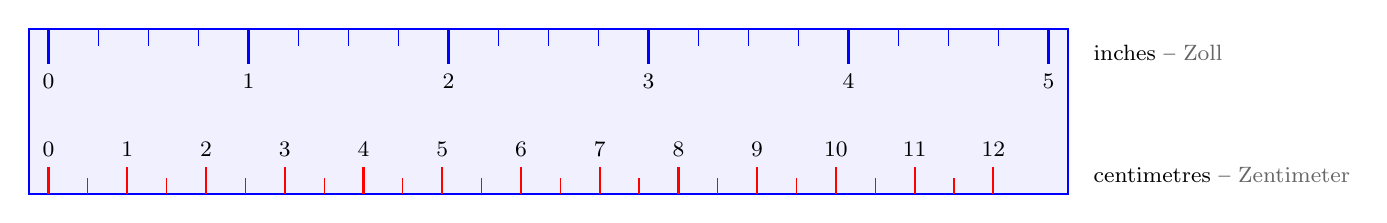
\begin{tikzpicture}[font=\footnotesize, x=1cm]
	\draw[blue, thick, fill=blue!6] (0,0) rectangle (13.2,2.1);
	\foreach \k in {0,...,5} {\draw[blue, thick] (0.25+2.54*\k,2.1) -- ++(0,-0.45) node[below, black] {\k};}
	\foreach \k in {0,...,19} {\draw[blue] (0.25+0.635*\k,2.1) -- ++(0,-0.22);}
	\foreach \k in {0,...,12} {\draw[red, thick] (0.25+\k,0) -- ++(0,0.35) node[above, black] {\k};}
	\foreach \k in {0,...,24} {\draw[red] (0.25+0.5*\k,0) -- ++(0,0.2);}
	\node[anchor=west] at (13.4,1.8) {inches -- \color{black!60}Zoll};
	\node[anchor=west] at (13.4,0.25) {centimetres -- \color{black!60}Zentimeter};
\end{tikzpicture}
\end{center}

\subsection*{Länge}
\begin{lesen}
\lies{$1\eh{in} = 2{,}54\eh{cm}$ \newline \footnotesize auch $1''$}{one inch \ipa{IntS} equals two point five four centimetres}{ein Zoll sind zwei Komma fünf vier Zentimeter}
\lies{$1\eh{ft} = 12\eh{in} = 30{,}48\eh{cm}$ \newline \footnotesize auch $1'$}{one foot (plural: feet) equals twelve inches}{ein Fuß sind zwölf Zoll}
\lies{$1\eh{yd} = 3\eh{ft} = 91{,}44\eh{cm}$}{one yard \ipa{jA:d} equals three feet}{ein Yard sind drei Fuß}
\lies{$1\eh{mi} = 1760\eh{yd} \approx 1{,}609\eh{km}$}{one mile equals one thousand seven hundred and sixty yards}{eine Meile sind eintausendsiebenhundertsechzig Yard}
\end{lesen}

\subsection*{Volumen und Masse}
\begin{lesen}
\lies{$1\eh{pt} \approx 568\eh{ml}$ (GB) \newline $1\eh{pt} \approx 473\eh{ml}$ (US)}{one pint \ipa{paInt}}{ein Pint}
\lies{$1\eh{gal} \approx 4{,}546\eh{l}$ (GB) \newline $1\eh{gal} \approx 3{,}785\eh{l}$ (US)}{one gallon \ipa{"g\ae l@n} equals eight pints}{eine Gallone sind acht Pints}
\lies{$1\eh{oz} \approx 28{,}35\eh{g}$}{one ounce \ipa{aUns}}{eine Unze}
\lies{$1\eh{lb} = 16\eh{oz} \approx 453{,}6\eh{g}$}{one pound \ipa{paUnd} equals sixteen ounces}{ein Pfund sind sechzehn Unzen}
\lies{$1\eh{st} = 14\eh{lb} \approx 6{,}35\eh{kg}$}{one stone equals fourteen pounds (used in Britain for body weight)}{ein Stone sind vierzehn Pfund (in Großbritannien für das Körpergewicht)}
\end{lesen}

\subsection*{Geschwindigkeit, Druck, Leistung, Energie}
\begin{lesen}
\lies{$1\eh{mph} \approx 1{,}609\eh{km/h}$}{one mile per hour}{eine Meile pro Stunde}
\lies{$1\eh{psi} \approx 6895\eh{Pa}$}{one pound per square inch}{ein Pfund pro Quadratzoll}
\lies{$1\eh{hp} \approx 746\eh{W}$}{one horsepower \ipa{"hO:spaU@}}{eine (britische) Pferdestärke; $1\eh{PS} \approx 735{,}5\eh{W}$}
\lies{$1\eh{Btu} \approx 1055\eh{J}$}{one British thermal unit}{eine britische Wärmeeinheit}
\lies{$1\eh{cal} \approx 4{,}19\eh{J}$}{one calorie \ipa{"k\ae l@ri}}{eine Kalorie}
\end{lesen}

\anmerkung{Vorsicht bei \textit{gallon} und \textit{pint}: Die britischen Einheiten sind etwa 20\,\%
größer als die amerikanischen. Körpergröße wird in \textit{feet} und \textit{inches} angegeben:
$5'\,11''$ -- \textit{five foot eleven}.}

\subsection*{Beispiele}

\begin{lesen}
\lies{$6\eh{ft} \approx 1{,}83\eh{m}$}{He is six feet tall, that is about one metre eighty-three.}{Er ist sechs Fuß groß, das sind etwa ein Meter dreiundachtzig.}
\lies{$70\eh{mph} \approx 113\eh{km/h}$}{The speed limit on British motorways is seventy miles per hour.}{Auf britischen Autobahnen gilt ein Tempolimit von siebzig Meilen pro Stunde.}
\lies{$27\eh{in} \approx 68{,}6\eh{cm}$}{a twenty-seven-inch monitor}{ein Siebenundzwanzig-Zoll-Monitor}
\lies{$32\eh{psi} \approx 2{,}2\eh{bar}$}{The tyre pressure should be thirty-two pounds per square inch.}{Der Reifendruck soll etwa zwei Komma zwei Bar betragen.}
\lies{$150\eh{lb} \approx 68\eh{kg}$}{one hundred and fifty pounds is about sixty-eight kilograms}{hundertfünfzig Pfund sind etwa achtundsechzig Kilogramm}
\end{lesen}

%--------------------------------------------------------------------------------------------------
\section{Temperaturskalen}

\begin{center}
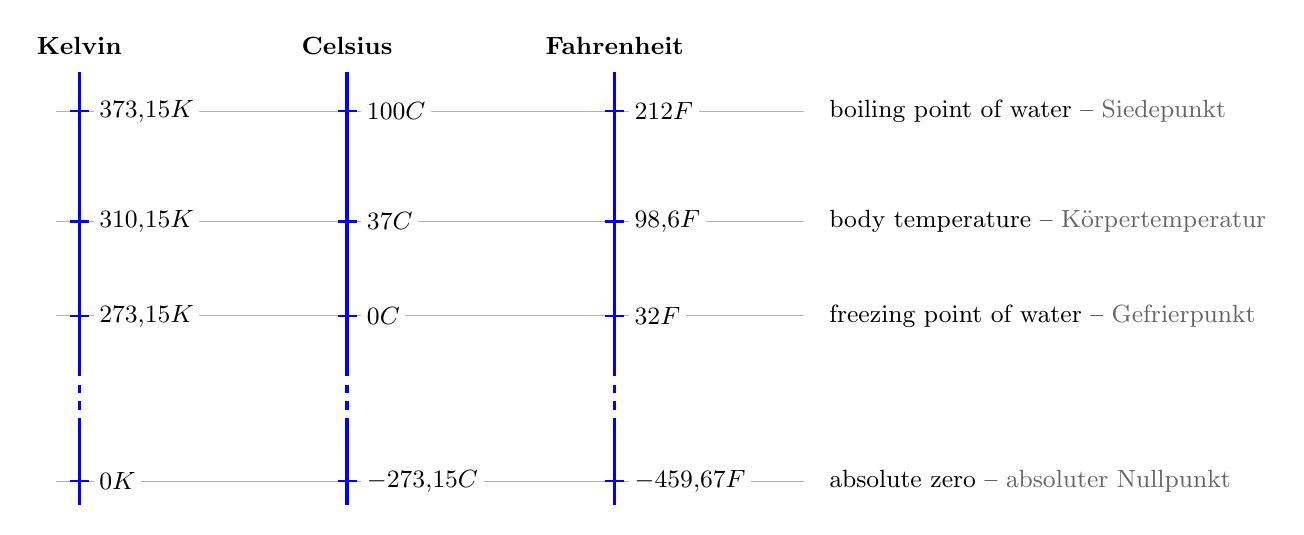
\begin{tikzpicture}[font=\small]
	\foreach \y in {0.3,2.4,3.6,5.0} {\draw[black!30, thin] (-0.3,\y) -- (9.2,\y);}
	\foreach \x/\name in {0/Kelvin, 3.4/Celsius, 6.8/Fahrenheit} {
		\draw[blue, very thick] (\x,0) -- (\x,1.0); \draw[blue, very thick, dashed] (\x,1.0) -- (\x,1.7); \draw[blue, very thick] (\x,1.7) -- (\x,5.5);
		\node[above, font=\small\bfseries] at (\x,5.6) {\name};
		\foreach \y in {0.3,2.4,3.6,5.0} {\draw[blue, thick] (\x-0.12,\y) -- (\x+0.12,\y);}}
	\foreach \y/\k/\c/\f in {0.3/0\eh{K}/-273{,}15\eh{\degree C}/-459{,}67\eh{\degree F}, 2.4/273{,}15\eh{K}/0\eh{\degree C}/32\eh{\degree F},
			3.6/310{,}15\eh{K}/37\eh{\degree C}/98{,}6\eh{\degree F}, 5.0/373{,}15\eh{K}/100\eh{\degree C}/212\eh{\degree F}} {
		\node[right, fill=white, inner sep=2pt, xshift=5pt] at (0,\y) {$\k$}; \node[right, fill=white, inner sep=2pt, xshift=5pt] at (3.4,\y) {$\c$};
		\node[right, fill=white, inner sep=2pt, xshift=5pt] at (6.8,\y) {$\f$};}
	\node[anchor=west] at (9.4,0.3) {absolute zero -- \color{black!60}absoluter Nullpunkt};
	\node[anchor=west] at (9.4,2.4) {freezing point of water -- \color{black!60}Gefrierpunkt};
	\node[anchor=west] at (9.4,3.6) {body temperature -- \color{black!60}Körpertemperatur};
	\node[anchor=west] at (9.4,5.0) {boiling point of water -- \color{black!60}Siedepunkt};
\end{tikzpicture}
\end{center}

\begin{lesen}
\lies{$\vartheta_C,\ \vartheta_F$}{the temperature in degrees Celsius \ipa{"selsi@s} and in degrees Fahrenheit \ipa{"f\ae r@nhaIt}}{die Temperatur in Grad Celsius und in Grad Fahrenheit}
\lies{$T$}{the absolute (thermodynamic) temperature in kelvin}{die absolute (thermodynamische) Temperatur in Kelvin}
\lies{$T = \vartheta_C + 273{,}15$}{To convert degrees Celsius into kelvin, add two hundred and seventy-three point one five.}{Zur Umrechnung von Grad Celsius in Kelvin addiert man zweihundertdreiundsiebzig Komma eins fünf.}
\lies{$\vartheta_F = \dfrac{9}{5} \cdot \vartheta_C + 32$}{To convert degrees Celsius into degrees Fahrenheit, multiply by nine fifths and add thirty-two.}{Zur Umrechnung von Grad Celsius in Grad Fahrenheit multipliziert man mit neun Fünfteln und addiert zweiunddreißig.}
\lies{$\vartheta_C = \dfrac{5}{9} \cdot (\vartheta_F - 32)$}{To convert degrees Fahrenheit into degrees Celsius, subtract thirty-two and multiply by five ninths.}{Zur Umrechnung von Grad Fahrenheit in Grad Celsius subtrahiert man zweiunddreißig und multipliziert mit fünf Neunteln.}
\lies{$\Delta T = 15\eh{K}$}{a temperature difference (a rise in temperature) of fifteen kelvin}{eine Temperaturdifferenz (ein Temperaturanstieg) von fünfzehn Kelvin}
\end{lesen}

\anmerkung{Die Umrechnungsformeln sind Zahlenwertgleichungen: Man setzt nur die Zahlenwerte ein.
Statt \textit{degrees Celsius} hört man im Alltag auch noch \textit{degrees centigrade}
\ipa{"sentIgreId}. Temperaturdifferenzen gibt man in Kelvin an.}

\subsection*{Beispiele}

\begin{lesen}
\lies{$68\eh{\degree F} \mathrel{\widehat{=}} 20\eh{\degree C}$}{Sixty-eight degrees Fahrenheit corresponds to twenty degrees Celsius: sixty-eight minus thirty-two is thirty-six; thirty-six times five ninths is twenty.}{Achtundsechzig Grad Fahrenheit entsprechen zwanzig Grad Celsius: achtundsechzig minus zweiunddreißig ist sechsunddreißig; sechsunddreißig mal fünf Neuntel ist zwanzig.}
\lies{$-40\eh{\degree C} \mathrel{\widehat{=}} -40\eh{\degree F}$}{At minus forty degrees the Celsius and the Fahrenheit scales show the same value.}{Bei minus vierzig Grad zeigen die Celsius- und die Fahrenheit-Skala denselben Wert.}
\lies{$-5\eh{\degree C}$}{minus five degrees Celsius \;/\; five degrees below zero}{minus fünf Grad Celsius \;/\; fünf Grad unter null}
\lies{$0\eh{K}$}{Absolute zero is the lowest possible temperature.}{Der absolute Nullpunkt ist die tiefste mögliche Temperatur.}
\end{lesen}

%--------------------------------------------------------------------------------------------------
\section{Formeln lesen: Mechanik}

\begin{lesen}
\lies{$v = \dfrac{s}{t}$}{$v$ equals $s$ over $t$: speed equals distance divided by time}{$v$ gleich $s$ durch $t$: Geschwindigkeit gleich Weg durch Zeit}
\lies{$a = \dfrac{\Delta v}{\Delta t}$}{$a$ equals delta $v$ over delta $t$: acceleration is the change in velocity divided by the time taken}{$a$ gleich Delta $v$ durch Delta $t$: Die Beschleunigung ist die Geschwindigkeitsänderung durch die dafür benötigte Zeit}
\lies{$s = \dfrac{1}{2} \cdot a \cdot t^2$}{$s$ equals a half $a$ $t$ squared}{$s$ gleich ein Halb $a$ $t$ Quadrat}
\lies{$F = m \cdot a$}{$F$ equals $m$ $a$: force equals mass times acceleration}{$F$ gleich $m$ mal $a$: Kraft gleich Masse mal Beschleunigung}
\lies{$F_G = m \cdot g$}{weight equals mass times the acceleration due to gravity}{Gewichtskraft gleich Masse mal Fallbeschleunigung}
\lies{$\varrho = \dfrac{m}{V}$}{rho equals $m$ over $V$: density equals mass divided by volume}{Rho gleich $m$ durch $V$: Dichte gleich Masse durch Volumen}
\lies{$p = \dfrac{F}{A}$}{$p$ equals $F$ over $A$: pressure equals force divided by area}{$p$ gleich $F$ durch $A$: Druck gleich Kraft durch Fläche}
\lies{$W = F \cdot s$}{work done equals force times distance (moved in the direction of the force)}{Arbeit gleich Kraft mal Weg (in Kraftrichtung)}
\lies{$E_{\mathrm{kin}} = \dfrac{1}{2} \cdot m \cdot v^2$}{kinetic energy equals a half $m$ $v$ squared}{kinetische Energie gleich ein Halb $m$ $v$ Quadrat}
\lies{$E_{\mathrm{pot}} = m \cdot g \cdot h$}{potential energy equals $m$ $g$ $h$}{potentielle Energie gleich $m$ $g$ $h$}
\lies{$P = \dfrac{W}{t}$}{power equals work done divided by time taken}{Leistung gleich Arbeit durch Zeit}
\lies{$F = G \cdot \dfrac{m_1 \cdot m_2}{r^2}$}{$F$ equals capital $G$ times $m$ one $m$ two over $r$ squared}{$F$ gleich groß $G$ mal $m$ eins mal $m$ zwei durch $r$ Quadrat}
\end{lesen}

\anmerkung{Einige Formelzeichen unterscheiden sich: Im Englischen steht meist $d$ oder $s$ für den
Weg (\textit{distance, displacement}), $k$ für die Federkonstante, $W$ für die Gewichtskraft
(\textit{weight}) und $u$ für die Anfangsgeschwindigkeit: $v = u + a\,t$.}

\subsection*{Beispiele}

\begin{lesen}
\lies{\textit{Gegeben -- gesucht}}{\textit{Given:} $m$ equals two kilograms, $a$ equals three metres per second squared. \textit{Find:} the force $F$.}{\textit{Gegeben:} $m$ gleich zwei Kilogramm, $a$ gleich drei Meter pro Sekunde zum Quadrat. \textit{Gesucht:} die Kraft $F$.}
\lies{$F = m \cdot a$ \newline $F = 2\eh{kg} \cdot 3\eh{m/s^2}$}{Write down the equation and substitute the values.}{Schreibe die Gleichung auf und setze die Werte ein.}
\lies{$F = 6\eh{N}$}{The force is six newtons.}{Die Kraft beträgt sechs Newton.}
\lies{$v = \dfrac{s}{t} \ \Rightarrow\ t = \dfrac{s}{v}$}{Rearrange the equation to make $t$ the subject \;/\; solve the equation for $t$.}{Stelle die Gleichung nach $t$ um \;/\; löse die Gleichung nach $t$ auf.}
\lies{$E_{\mathrm{kin}} = \frac12 \cdot 1000\eh{kg} \cdot (20\eh{m/s})^2$ \newline $E_{\mathrm{kin}} = 200\eh{kJ}$}{A car with a mass of one thousand kilograms travelling at twenty metres per second has a kinetic energy of two hundred kilojoules.}{Ein Auto der Masse eintausend Kilogramm hat bei zwanzig Meter pro Sekunde eine kinetische Energie von zweihundert Kilojoule.}
\end{lesen}

%--------------------------------------------------------------------------------------------------
\section{Formeln lesen: Elektrizitätslehre}

\begin{center}
\begin{circuitikz}[font=\footnotesize]
	\draw (0,0) to[battery1, l=$U$] (0,2.6) to[rmeter, t=A] (2.6,2.6) to[lamp, l=$L_1$] (5.2,2.6) to[R, l=$R$] (5.2,0) to[nos] (2.6,0) -- (0,0);
	\draw (5.2,2.6) -- (6.7,2.6) to[rmeter, t=V] (6.7,0) -- (5.2,0);
	\fill (5.2,2.6) circle (1.6pt) (5.2,0) circle (1.6pt);
	\node[anchor=west, align=left] at (8,2.5) {\sz{battery1}\; cell, battery -- \color{black!60}Batterie};
	\node[anchor=west, align=left] at (8,1.95) {\sz{nos}\; switch -- \color{black!60}Schalter};
	\node[anchor=west, align=left] at (8,1.4) {\sz{lamp}\; lamp -- \color{black!60}Lampe};
	\node[anchor=west, align=left] at (8,0.85) {\sz{R}\; resistor -- \color{black!60}Widerstand};
	\node[anchor=west, align=left] at (8,0.3) {\sz{rmeter, t=A}\; ammeter -- \color{black!60}Strommesser};
	\node[anchor=west, align=left] at (8,-0.25) {\sz{rmeter, t=V}\; voltmeter -- \color{black!60}Spannungsmesser};
\end{circuitikz}
\end{center}

\begin{lesen}
\lies{$I = \dfrac{Q}{t}$}{$I$ equals $Q$ over $t$: current is the charge flowing per unit time}{$I$ gleich $Q$ durch $t$: Die Stromstärke ist die pro Zeit fließende Ladung}
\lies{$U = R \cdot I$ \newline \footnotesize engl. $V = I\,R$}{$V$ equals $I$ $R$: voltage equals current times resistance (Ohm's law)}{$U$ gleich $R$ mal $I$: Spannung gleich Widerstand mal Stromstärke (ohmsches Gesetz)}
\lies{$P = U \cdot I$ \newline \footnotesize engl. $P = I\,V$}{power equals current times voltage}{Leistung gleich Spannung mal Stromstärke}
\lies{$E = U \cdot I \cdot t$}{energy transferred equals voltage times current times time}{elektrische Energie gleich Spannung mal Stromstärke mal Zeit}
\lies{$R_{\mathrm{ges}} = R_1 + R_2$}{in series: the total resistance equals $R$ one plus $R$ two}{Reihenschaltung: Der Gesamtwiderstand ist gleich $R$ eins plus $R$ zwei}
\lies{$\dfrac{1}{R_{\mathrm{ges}}} = \dfrac{1}{R_1} + \dfrac{1}{R_2}$}{in parallel: one over the total resistance equals one over $R$ one plus one over $R$ two}{Parallelschaltung: eins durch $R$ gesamt gleich eins durch $R$ eins plus eins durch $R$ zwei}
\lies{$C = \dfrac{Q}{U}$}{capacitance equals charge divided by voltage}{Kapazität gleich Ladung durch Spannung}
\lies{$\dfrac{U_1}{U_2} = \dfrac{N_1}{N_2}$}{the ratio of the voltages equals the ratio of the numbers of turns (transformer equation)}{die Spannungen verhalten sich wie die Windungszahlen (Transformatorgleichung)}
\end{lesen}

\anmerkung{Im Englischen ist das Formelzeichen für die Spannung $V$ (\textit{voltage}), nicht $U$ --
Zeichen und Einheit sehen dann gleich aus: $V = 12\eh{V}$. Man sagt \textit{the voltage across
the lamp} (an der Lampe) und \textit{the current through the lamp} (durch die Lampe).}

\subsection*{Beispiele}

\begin{lesen}
\lies{$I = \dfrac{U}{R} = \dfrac{6\eh{V}}{12\eh{\Omega}} = 0{,}5\eh{A}$}{A six-volt battery is connected to a twelve-ohm resistor. The current is nought point five amperes.}{An eine Sechs-Volt-Batterie wird ein Zwölf-Ohm-Widerstand angeschlossen. Die Stromstärke beträgt null Komma fünf Ampere.}
\lies{$R_{\mathrm{ges}} = 100\eh{\Omega} + 220\eh{\Omega} = 320\eh{\Omega}$}{Two resistors of one hundred ohms and two hundred and twenty ohms in series have a total resistance of three hundred and twenty ohms.}{Zwei Widerstände von hundert Ohm und zweihundertzwanzig Ohm in Reihe haben einen Gesamtwiderstand von dreihundertzwanzig Ohm.}
\lies{$R_{\mathrm{ges}} = \dfrac{60\eh{\Omega} \cdot 30\eh{\Omega}}{60\eh{\Omega} + 30\eh{\Omega}} = 20\eh{\Omega}$}{Sixty ohms and thirty ohms in parallel give a total resistance of twenty ohms.}{Sechzig Ohm und dreißig Ohm parallel ergeben einen Gesamtwiderstand von zwanzig Ohm.}
\lies{$E = 2\eh{kW} \cdot 0{,}5\eh{h} = 1\eh{kWh}$}{A two-kilowatt kettle switched on for half an hour transfers one kilowatt-hour of energy.}{Ein Wasserkocher mit zwei Kilowatt, der eine halbe Stunde eingeschaltet ist, wandelt eine Kilowattstunde Energie um.}
\lies{Schalter}{Close the switch: the circuit is complete and the lamp lights up. Open the switch: the lamp goes out.}{Schließe den Schalter: Der Stromkreis ist geschlossen und die Lampe leuchtet. Öffne den Schalter: Die Lampe erlischt.}
\end{lesen}

%--------------------------------------------------------------------------------------------------
\section{Formeln lesen: Wärme, Wellen, Optik und Atome}

\begin{lesen}
\lies{$Q = c \cdot m \cdot \Delta T$}{$Q$ equals $c$ $m$ delta $T$: heat equals specific heat capacity times mass times temperature change}{$Q$ gleich $c$ mal $m$ mal Delta $T$: Wärme gleich spezifische Wärmekapazität mal Masse mal Temperaturänderung}
\lies{$\dfrac{p_1 \cdot V_1}{T_1} = \dfrac{p_2 \cdot V_2}{T_2}$}{$p$ one $V$ one over $T$ one equals $p$ two $V$ two over $T$ two}{$p$ eins mal $V$ eins durch $T$ eins gleich $p$ zwei mal $V$ zwei durch $T$ zwei}
\lies{$f = \dfrac{1}{T}$}{frequency equals one over the period}{Frequenz gleich eins durch Periodendauer}
\lies{$c = \lambda \cdot f$ \newline \footnotesize engl. $v = f\,\lambda$}{wave speed equals frequency times wavelength \;/\; $v$ equals $f$ lambda}{Ausbreitungsgeschwindigkeit gleich Wellenlänge mal Frequenz \;/\; $c$ gleich Lambda mal $f$}
\lies{$T = 2\pi \cdot \sqrt{\dfrac{l}{g}}$}{$T$ equals two pi times the square root of $l$ over $g$}{$T$ gleich zwei pi mal Wurzel aus $l$ durch $g$}
\lies{$\dfrac{1}{f} = \dfrac{1}{g} + \dfrac{1}{b}$ \newline \footnotesize engl. $\frac{1}{f} = \frac{1}{u} + \frac{1}{v}$}{one over $f$ equals one over $u$ plus one over $v$ (the lens equation)}{eins durch $f$ gleich eins durch $g$ plus eins durch $b$ (die Linsengleichung)}
\lies{$n = \dfrac{\sin\alpha}{\sin\beta}$}{the refractive index equals sine alpha over sine beta \;/\; sine $i$ over sine $r$}{die Brechzahl ist gleich Sinus Alpha durch Sinus Beta}
\lies{$E = h \cdot f$}{$E$ equals $h$ $f$: the energy of a photon equals the Planck constant times the frequency}{$E$ gleich $h$ mal $f$: Die Energie eines Photons ist das plancksche Wirkungsquantum mal die Frequenz}
\lies{$E = m \cdot c^2$}{$E$ equals $m$ $c$ squared}{$E$ gleich $m$ $c$ Quadrat}
\lies{$N = N_0 \cdot \left(\dfrac{1}{2}\right)^{t/T_{1/2}}$}{$N$ equals $N$ nought times one half to the power of $t$ over the half-life}{$N$ gleich $N$ null mal ein Halb hoch $t$ durch die Halbwertszeit}
\lies{$^{238}_{\ 92}\mathrm{U}$}{uranium-two three eight: mass number two hundred and thirty-eight, atomic number ninety-two}{Uran-238: Massenzahl zweihundertachtunddreißig, Kernladungszahl zweiundneunzig}
\end{lesen}

\subsection*{Beispiele}

\begin{lesen}
\lies{$\lambda = \dfrac{c}{f} = \dfrac{3 \cdot 10^8\eh{m/s}}{100\eh{MHz}} = 3\eh{m}$}{A radio station broadcasts at one hundred megahertz. The wavelength is three metres.}{Ein Radiosender sendet mit hundert Megahertz. Die Wellenlänge beträgt drei Meter.}
\lies{$Q = 0{,}5\eh{kg} \cdot 4{,}19\eh{\tfrac{kJ}{kg \cdot K}} \cdot 80\eh{K}$ \newline $Q \approx 168\eh{kJ}$}{About one hundred and sixty-eight kilojoules are needed to heat half a kilogram of water from twenty to one hundred degrees Celsius.}{Um ein halbes Kilogramm Wasser von zwanzig auf hundert Grad Celsius zu erwärmen, sind etwa hundertachtundsechzig Kilojoule nötig.}
\lies{$N = N_0 \cdot \left(\frac12\right)^3 = \dfrac{N_0}{8}$}{After three half-lives one eighth of the original nuclei are left.}{Nach drei Halbwertszeiten ist noch ein Achtel der ursprünglichen Kerne vorhanden.}
\lies{$n = \dfrac{c_0}{c} = \dfrac{3{,}00 \cdot 10^8}{2{,}25 \cdot 10^8} \approx 1{,}33$}{The refractive index of water is about one point three three.}{Die Brechzahl von Wasser beträgt etwa eins Komma drei drei.}
\end{lesen}

%--------------------------------------------------------------------------------------------------
\section{Experimente beschreiben}

\begin{center}
\begin{tikzpicture}[font=\small]
	\draw[black, line width=2.5pt] (-1.3,0) -- (1.2,0);
	\draw[black, line width=2pt] (-0.8,0) -- (-0.8,5.2); \draw[black, line width=2pt] (-0.8,4.8) -- (1.9,4.8);
	\draw[blue, thick, decorate, decoration={zigzag, segment length=5pt, amplitude=5pt}] (1.5,4.8) -- (1.5,2.5);
	\draw[blue, thick] (1.5,2.5) -- (1.5,2.2); \filldraw[fill=blue!20, draw=blue, very thick] (1.15,1.5) rectangle (1.85,2.2);
	\draw[thick, fill=yellow!20] (2.4,0.3) rectangle (2.8,5.0); \foreach \y in {0.5,0.8,...,4.9} {\draw (2.4,\y) -- (2.55,\y);}
	\draw[red, thick, -{Stealth}] (1.5,1.5) -- (1.5,0.5) node[left] {$\vec{F}_G$};
	\node[anchor=west, align=left] (a) at (4.2,4.7) {clamp stand -- \color{black!60}Stativ};
	\node[anchor=west, align=left] (b) at (4.2,3.8) {spring -- \color{black!60}Feder};
	\node[anchor=west, align=left] (c) at (4.2,2.9) {ruler -- \color{black!60}Lineal};
	\node[anchor=west, align=left] (d) at (4.2,2.0) {mass (slotted masses) -- \color{black!60}Massestück};
	\node[anchor=west, align=left] (e) at (4.2,1.1) {weight (force) -- \color{black!60}Gewichtskraft};
	\draw[-{Stealth}, thin] (a.west) -- (1.0,4.9); \draw[-{Stealth}, thin] (b.west) -- (1.75,3.7); \draw[-{Stealth}, thin] (c.west) -- (2.85,2.9);
	\draw[-{Stealth}, thin] (d.west) -- (1.95,1.9); \draw[-{Stealth}, thin] (e.west) -- (1.65,1.0);
\end{tikzpicture}
\end{center}

Die Teile eines Versuchsprotokolls (\textit{lab report}):

\begin{lesen}
\lies{\textbf{Aufgabe}}{\textbf{Aim:} To investigate how the extension of a spring depends on the force applied.}{Untersuche, wie die Verlängerung einer Feder von der wirkenden Kraft abhängt.}
\lies{\textbf{Vermutung}}{\textbf{Hypothesis / Prediction:} The greater the force, the greater the extension.}{Je größer die Kraft, desto größer die Verlängerung.}
\lies{\textbf{Geräte}}{\textbf{Apparatus:} clamp stand, spring, slotted masses, ruler}{Stativ, Feder, Massestücke, Lineal}
\lies{\textbf{Durchführung}}{\textbf{Method:} Set up the apparatus as shown in the diagram. Measure the length of the unloaded spring. Add the masses one at a time and record the length of the spring each time.}{Baue den Versuch wie in der Skizze auf. Miss die Länge der unbelasteten Feder. Hänge nacheinander die Massestücke an und notiere jeweils die Länge der Feder.}
\lies{\textbf{Messwerte}}{\textbf{Results:} Record your readings in a table.}{Trage die Messwerte in eine Tabelle ein.}
\lies{\textbf{Auswertung}}{\textbf{Analysis / Conclusion:} Plot a graph of force against extension. The graph is a straight line through the origin, so the force is directly proportional to the extension.}{Zeichne ein Kraft-Verlängerungs-Diagramm. Der Graph ist eine Ursprungsgerade, also ist die Kraft proportional zur Verlängerung.}
\lies{\textbf{Fehlerbetrachtung}}{\textbf{Evaluation:} Sources of error are reading the ruler (parallax error) and the oscillation of the spring.}{Fehlerquellen sind das Ablesen am Lineal (Parallaxenfehler) und das Schwingen der Feder.}
\end{lesen}

\subsection*{Beispiele}

\begin{lesen}
\lies{Variablen}{Change only one variable at a time and keep all the other variables constant (a fair test).}{Ändere immer nur eine Größe und halte alle anderen Größen konstant.}
\lies{Messen}{Measure the time for ten oscillations and divide by ten.}{Miss die Zeit für zehn Schwingungen und dividiere durch zehn.}
\lies{Wiederholen}{Repeat each measurement three times and calculate the mean.}{Wiederhole jede Messung dreimal und berechne den Mittelwert.}
\lies{Beobachten}{What do you observe? -- The lamp gets brighter as the voltage increases.}{Was beobachtest du? -- Die Lampe leuchtet heller, wenn die Spannung steigt.}
\lies{Sicherheit}{Safety: wear safety goggles. Do not look directly into the laser beam.}{Sicherheit: Trage eine Schutzbrille. Blicke nicht direkt in den Laserstrahl.}
\end{lesen}

%--------------------------------------------------------------------------------------------------
\section{Diagramme beschreiben}

\begin{center}
\begin{tikzpicture}[font=\small, scale=1.05]
	\draw[black!15, very thin, step=0.5] (0,0) grid (6,4);
	\draw[achse] (-0.3,0) -- (6.5,0) node[right] {$s$ in cm}; \draw[achse] (0,-0.3) -- (0,4.5) node[above] {$F$ in N};
	\foreach \x in {1,...,6} {\node[below, font=\footnotesize] at (\x,0) {\x};}
	\foreach \y/\l in {1/0{,}5, 2/1{,}0, 3/1{,}5, 4/2{,}0} {\node[left, font=\footnotesize] at (0,\y) {$\l$};}
	\draw[red, thick] (0,0) -- (6.2,4.03);
	\foreach \x/\y in {1/0.75, 2/1.2, 3/2.05, 4/2.5, 5/3.35, 6/3.85} {\draw[blue, very thick] (\x-0.1,\y-0.1) -- (\x+0.1,\y+0.1) (\x-0.1,\y+0.1) -- (\x+0.1,\y-0.1);}
	\draw[black!70] (2,1.3) -- (5,1.3) node[midway, below, font=\footnotesize] {$\Delta s$} -- (5,3.25) node[midway, right, font=\footnotesize] {$\Delta F$};
	\node[anchor=west, align=left] (a) at (7.6,3.9) {line of best fit -- \color{black!60}Ausgleichsgerade};
	\node[anchor=west, align=left] (b) at (7.6,3.1) {data point (reading) -- \color{black!60}Messpunkt};
	\node[anchor=west, align=left] (c) at (7.6,2.3) {gradient triangle -- \color{black!60}Anstiegsdreieck};
	\node[anchor=west, align=left] (d) at (7.6,1.5) {$x$-axis: independent variable\\\color{black!60}Rechtsachse: unabhängige Größe};
	\node[anchor=west, align=left] (e) at (7.6,0.5) {origin -- \color{black!60}Koordinatenursprung};
	\draw[-{Stealth}, thin] (a.west) -- (5.9,3.9); \draw[-{Stealth}, thin] (b.west) -- (5.2,3.3); \draw[-{Stealth}, thin] (c.west) -- (5.15,2.3);
	\draw[-{Stealth}, thin] (e.west) -- (0.15,0.1);
\end{tikzpicture}
\end{center}

\begin{lesen}
\lies{Achsen}{The extension is plotted on the $x$-axis (horizontal axis), the force on the $y$-axis (vertical axis).}{Auf der Rechtsachse ist die Verlängerung abgetragen, auf der Hochachse die Kraft.}
\lies{Auftragen}{Plot a graph of force against extension \;/\; plot $F$ against $s$.}{Zeichne ein $F$-$s$-Diagramm \;/\; trage $F$ über $s$ auf.}
\lies{Gerade}{The graph is a straight line through the origin: $F$ is directly proportional to $s$.}{Der Graph ist eine Ursprungsgerade: $F$ ist proportional zu $s$.}
\lies{$D = \dfrac{\Delta F}{\Delta s}$}{The gradient (slope) of the line gives the spring constant.}{Der Anstieg der Geraden ergibt die Federkonstante.}
\lies{Verlauf}{The curve rises steeply at first and then levels off.}{Die Kurve steigt zunächst steil an und flacht dann ab.}
\lies{Verlauf}{The current increases \;/\; decreases \;/\; remains constant as the voltage increases.}{Die Stromstärke steigt \;/\; sinkt \;/\; bleibt konstant, wenn die Spannung zunimmt.}
\lies{Fläche}{The area under a velocity–time graph gives the distance travelled.}{Die Fläche unter dem Graphen im $v$-$t$-Diagramm entspricht dem zurückgelegten Weg.}
\lies{Ausreißer}{This reading is an anomalous result (an outlier); it is ignored when drawing the line of best fit.}{Dieser Messwert ist ein Ausreißer; er wird beim Zeichnen der Ausgleichsgeraden nicht berücksichtigt.}
\end{lesen}

\subsection*{Beispiele}

\begin{lesen}
\lies{$D = \dfrac{1{,}0\eh{N}}{3{,}1\eh{cm}} \approx 32\eh{N/m}$}{From the gradient triangle the spring constant is about thirty-two newtons per metre.}{Aus dem Anstiegsdreieck ergibt sich eine Federkonstante von etwa zweiunddreißig Newton pro Meter.}
\lies{\skST}{The distance–time graph is a straight line: the object moves at constant speed.}{Das Weg-Zeit-Diagramm ist eine Gerade: Der Körper bewegt sich mit konstanter Geschwindigkeit.}
\lies{\skVT}{The velocity increases uniformly with time: the acceleration is constant.}{Die Geschwindigkeit nimmt gleichmäßig mit der Zeit zu: Die Beschleunigung ist konstant.}
\lies{\skAntiprop}{The pressure is inversely proportional to the volume: if the volume is halved, the pressure doubles.}{Der Druck ist umgekehrt proportional zum Volumen: Wird das Volumen halbiert, verdoppelt sich der Druck.}
\lies{\skZerfall}{The number of undecayed nuclei decreases exponentially with time.}{Die Anzahl der noch nicht zerfallenen Kerne nimmt exponentiell mit der Zeit ab.}
\end{lesen}

%--------------------------------------------------------------------------------------------------
\section{Griechische Buchstaben in der Physik}

\begin{center}
{\small\renewcommand{\arraystretch}{1.25}
\begin{tabular}{@{}c l l l@{}}
	\toprule
	\textbf{Zeichen} & \textbf{Englisch} & \textbf{steht für (englisch)} & \textbf{steht für (deutsch)} \\ \midrule
	$\alpha$ & alpha \ipa{"\ae lf@} & angle; alpha particle & Winkel; Alphateilchen \\
	$\beta$ & beta \ipa{"bi:t@} & angle; beta particle & Winkel; Betateilchen \\
	$\gamma$ & gamma \ipa{"g\ae m@} & gamma radiation & Gammastrahlung \\
	$\Delta$ & delta \ipa{"delt@} & change in, difference & Änderung, Differenz \\
	$\varepsilon$ & epsilon \ipa{"epsIl6n} & permittivity & Permittivität (Dielektrizitätszahl) \\
	$\eta$ & eta \ipa{"i:t@} & efficiency & Wirkungsgrad \\
	$\vartheta$ & theta \ipa{"Ti:t@} & temperature; angle & Temperatur; Winkel \\
	$\lambda$ & lambda \ipa{"l\ae md@} & wavelength; decay constant & Wellenlänge; Zerfallskonstante \\
	$\mu$ & mu \ipa{mju:} & coefficient of friction; micro- & Reibungszahl; Mikro- \\
	$\varrho$ & rho \ipa{r@U} & density; resistivity & Dichte; spezifischer Widerstand \\
	$\sigma$ & sigma \ipa{"sIgm@} & stress; conductivity & mechanische Spannung; Leitfähigkeit \\
	$\tau$ & tau \ipa{taU} & time constant & Zeitkonstante \\
	$\varphi$ & phi \ipa{faI} & angle; phase; potential & Winkel; Phase; Potential \\
	$\Phi$ & capital phi & magnetic flux & magnetischer Fluss \\
	$\omega$ & omega \ipa{"@UmIg@} & angular velocity & Winkelgeschwindigkeit \\
	$\Omega$ & capital omega & ohm & Ohm \\
	\bottomrule
\end{tabular}}
\end{center}

\subsection*{Beispiele}

\begin{lesen}
\lies{$\Delta T = T_2 - T_1$}{delta $T$ equals $T$ two minus $T$ one: the change in temperature}{Delta $T$ gleich $T$ zwei minus $T$ eins: die Temperaturänderung}
\lies{$\eta = 0{,}85$}{eta equals nought point eight five: the efficiency is eighty-five per cent}{Eta gleich null Komma acht fünf: Der Wirkungsgrad beträgt fünfundachtzig Prozent}
\lies{$\lambda = 589\eh{nm}$}{lambda equals five hundred and eighty-nine nanometres (yellow sodium light)}{Lambda gleich fünfhundertneunundachtzig Nanometer (gelbes Natriumlicht)}
\lies{$\varrho = 7{,}87\eh{g/cm^3}$}{rho equals seven point eight seven grams per cubic centimetre (the density of iron)}{Rho gleich sieben Komma acht sieben Gramm pro Kubikzentimeter (die Dichte von Eisen)}
\lies{$R = 47\eh{\Omega}$}{$R$ equals forty-seven ohms}{$R$ gleich siebenundvierzig Ohm}
\end{lesen}
